\documentclass[sigplan,nonacm]{acmart}

\settopmatter{printacmref=false}
\setcopyright{none}
\renewcommand\footnotetextcopyrightpermission[1]{}
\usepackage{amsmath}
\usepackage{booktabs}
\usepackage{graphicx}
\usepackage{xurl}
\usepackage{listings}
\usepackage{placeins}
\graphicspath{{figures/}{report/figures/}}
\emergencystretch=2em
\lstset{basicstyle=\ttfamily\scriptsize,breaklines=true,columns=fullflexible}
\setlength{\textfloatsep}{10pt plus 2pt minus 2pt}
\setlength{\floatsep}{8pt plus 2pt minus 2pt}

\title{Length-Aware Request Scheduling for vLLM}
\subtitle{Performance and Fairness Trade-offs in LLM Serving}
\author{Carleano Chang (poching2)}
\author{Christine Liou (ycliou2)}
\renewcommand{\shortauthors}{Chang and Liou}

\begin{document}
\begin{abstract}
LLM inference requests vary in prompt and generation length. We study
whether sorting vLLM's waiting queues by estimated length improves
responsiveness, and whether waiting-time aging protects long requests.
Across 380 audited single-GPU runs, the gains depended on congestion and
admission capacity. In balanced traffic at 30 requests/s and a four-sequence
cap, Queue-Only reduced mean short-request P95 time to first token from
141.53 to 1.81 seconds. At 5 requests/s and a 16-sequence cap, all three
main policies served both classes with mean P95 below 60 milliseconds.
In a sustained-short stress test, both length-aware policies delayed
59 of 60 long probes until after the last short request was sent.
The results identify a useful operating regime for length-aware
ordering and a fairness failure that smooth aging did not resolve.
\end{abstract}

\keywords{LLM serving, vLLM, scheduling, tail latency, fairness}
\maketitle
\pagestyle{plain}
\thispagestyle{plain}

\section{Introduction}

Interactive LLM services process requests with widely varying input
and output lengths. When GPU capacity is limited, requests compete
for admission, and a long request can delay a much shorter one.
vLLM improves serving efficiency using PagedAttention and continuous
batching~\cite{kwon2023efficient}, while admission order still
determines which waiting requests reach a batch.

We ask when lightweight length-aware queue ordering improves short
tail latency and how the improvement affects long-request latency
and throughput. We implement two scheduler variants in vLLM,
compare them with its native first-come, first-served (FCFS) scheduler,
and vary load, request mix, and admission capacity. We also profile
the cost of queue sorting and stress-test long requests under
sustained arrivals of short work.

\section{Related Work}

PagedAttention improves KV-cache management in vLLM, and Orca
introduced iteration-level scheduling and selective
batching~\cite{kwon2023efficient,yu2022orca}. Sarathi-Serve uses
chunked prefill and scheduling to address the throughput--latency
trade-off~\cite{agrawal2024sarathi}. Llumnix addresses cluster-scale
scheduling through live migration~\cite{sun2024llumnix}. Bari
et al. study routing and scheduling with a model of inference
service and workload knowledge~\cite{bari2025optimal}.
Our experiments study a narrower intervention within a single
vLLM server, where waiting-queue ordering changes while the
admission and execution engine stays in place.

\section{Scheduling and Implementation}

For request $i$, let $p_i$ be its prompt-token count, $o_i$ its
requested maximum generation length, and $a_i$ its arrival time.
We estimate its size as $L_i=p_i+o_i$ and elapsed waiting time as
$w_i(t)=\max(0,t-a_i)$. Prefill and decoding have different costs,
so $L_i$ is a proxy for service demand.

\textbf{Native FCFS} uses vLLM's default queue ordering.
\textbf{Queue-Only} orders waiting requests by increasing $L_i$.
\textbf{Aging} adjusts the score as
\begin{equation}
P_i(t)=\frac{L_i}{1+\alpha w_i(t)},\qquad \alpha=0.5
\label{eq:aging}
\end{equation}
for the main comparison. Lower scores receive higher priority
and the arrival timestamp breaks ties. Appendix~\ref{app:example}
gives a worked example.

Both custom policies subclass vLLM's \texttt{AsyncScheduler}.
Each call sorts the waiting and skipped-waiting queues independently and
then calls the native scheduler. vLLM retains control of batch membership,
memory constraints and queue selection. Sorting costs $O(n\log n)$ in the
worst case for a queue of $n$ requests. Aging recomputes scores each step
because relative priorities can change over time. A profiling variant
skips clearing and rebuilding an Aging queue when the stable sort leaves
its order unchanged. Its priority rule is identical.

We also test native priority using tokenized prompt length plus the
maximum output length as the API priority, prompt-only ordering,
and per-request uniform multiplicative noise in $[0.7,1.3]$. Aging
variants use $\alpha\in\{1,2,5,10\}$. Wait Promotion prioritizes
requests after 10 seconds within their queue, and highest response
ratio next (HRRN) orders by $w_i/L_i$. These rules affect queue order.
Admission remains subject to available capacity.

\section{Experimental Method}

\paragraph{Environment.}
Each run used one NVIDIA L40S on Modal, vLLM 0.26.0 and
Qwen2.5-0.5B-Instruct, with a 2,048-token model limit,
FP16, asynchronous scheduling, eager execution, and prefix caching
disabled. The benchmark client and server ran in the same container.
We restarted the server per run and issued one short and one long warm-up
request before collecting measurements. The concurrency limit
\texttt{max-num-seqs} was four unless varied explicitly.
An earlier RTX 5090 exploration informed the choice of policies.

\paragraph{Design.}
Each trace contains 900 requests. In the two-size workloads,
short requests use approximately 32 prompt tokens and 16 output tokens,
and long requests use 256 and 128. The short-heavy mix has 813 short
requests and the balanced mix has 455. We send requests at
Poisson target rates of 2, 5, 10, 15, 20 and 30 requests/s.
A block uses the same trace for all compared policies, with a randomized
policy order. Each condition has five such repetitions.
Table~\ref{tab:design} enumerates the data used in this report.

\begin{table}[t]
\centering
\caption{Audited Modal runs used in the report. Each condition has five repetitions.}
\label{tab:design}
\small
\begin{tabular}{@{}lr@{}}
\toprule
Experiment & Runs \\
\midrule
Three policies, two mixes, six rates at cap 4 & 180 \\
Balanced at 5 requests/s, caps 16, 64, 256 & 45 \\
Nine policy variants, balanced at 5 requests/s & 45 \\
Scheduler profiling, balanced at 30 requests/s & 20 \\
Three ratio mixes, continuous lengths and bursts & 75 \\
Long probes during sustained short arrivals & 15 \\
\midrule
Total & 380 \\
\bottomrule
\end{tabular}
\end{table}

\paragraph{Metrics and audit.}
Client TTFT measures time from send to first streamed text. We also
record end-to-end latency and generated tokens per second over the
measurement window. We report means of per-run percentiles and show
individual repetitions. Server queue time uses vLLM histogram deltas
after warm-up. Traced batches also record per-request
queue time from OpenTelemetry spans. A valid run must match the
expected request IDs, completion lengths, and timestamp ordering,
and reproduce its stored summary from the raw trace.
Failed attempts are preserved. One main run and four workload-sweep
attempts failed before successful replays. An initial profiling batch
lacked CPU timing records and was rerun with direct snapshot output.
Smoke tests and calibration are outside Table~\ref{tab:design}.

\section{Results}

\begin{figure*}[t]
\centering
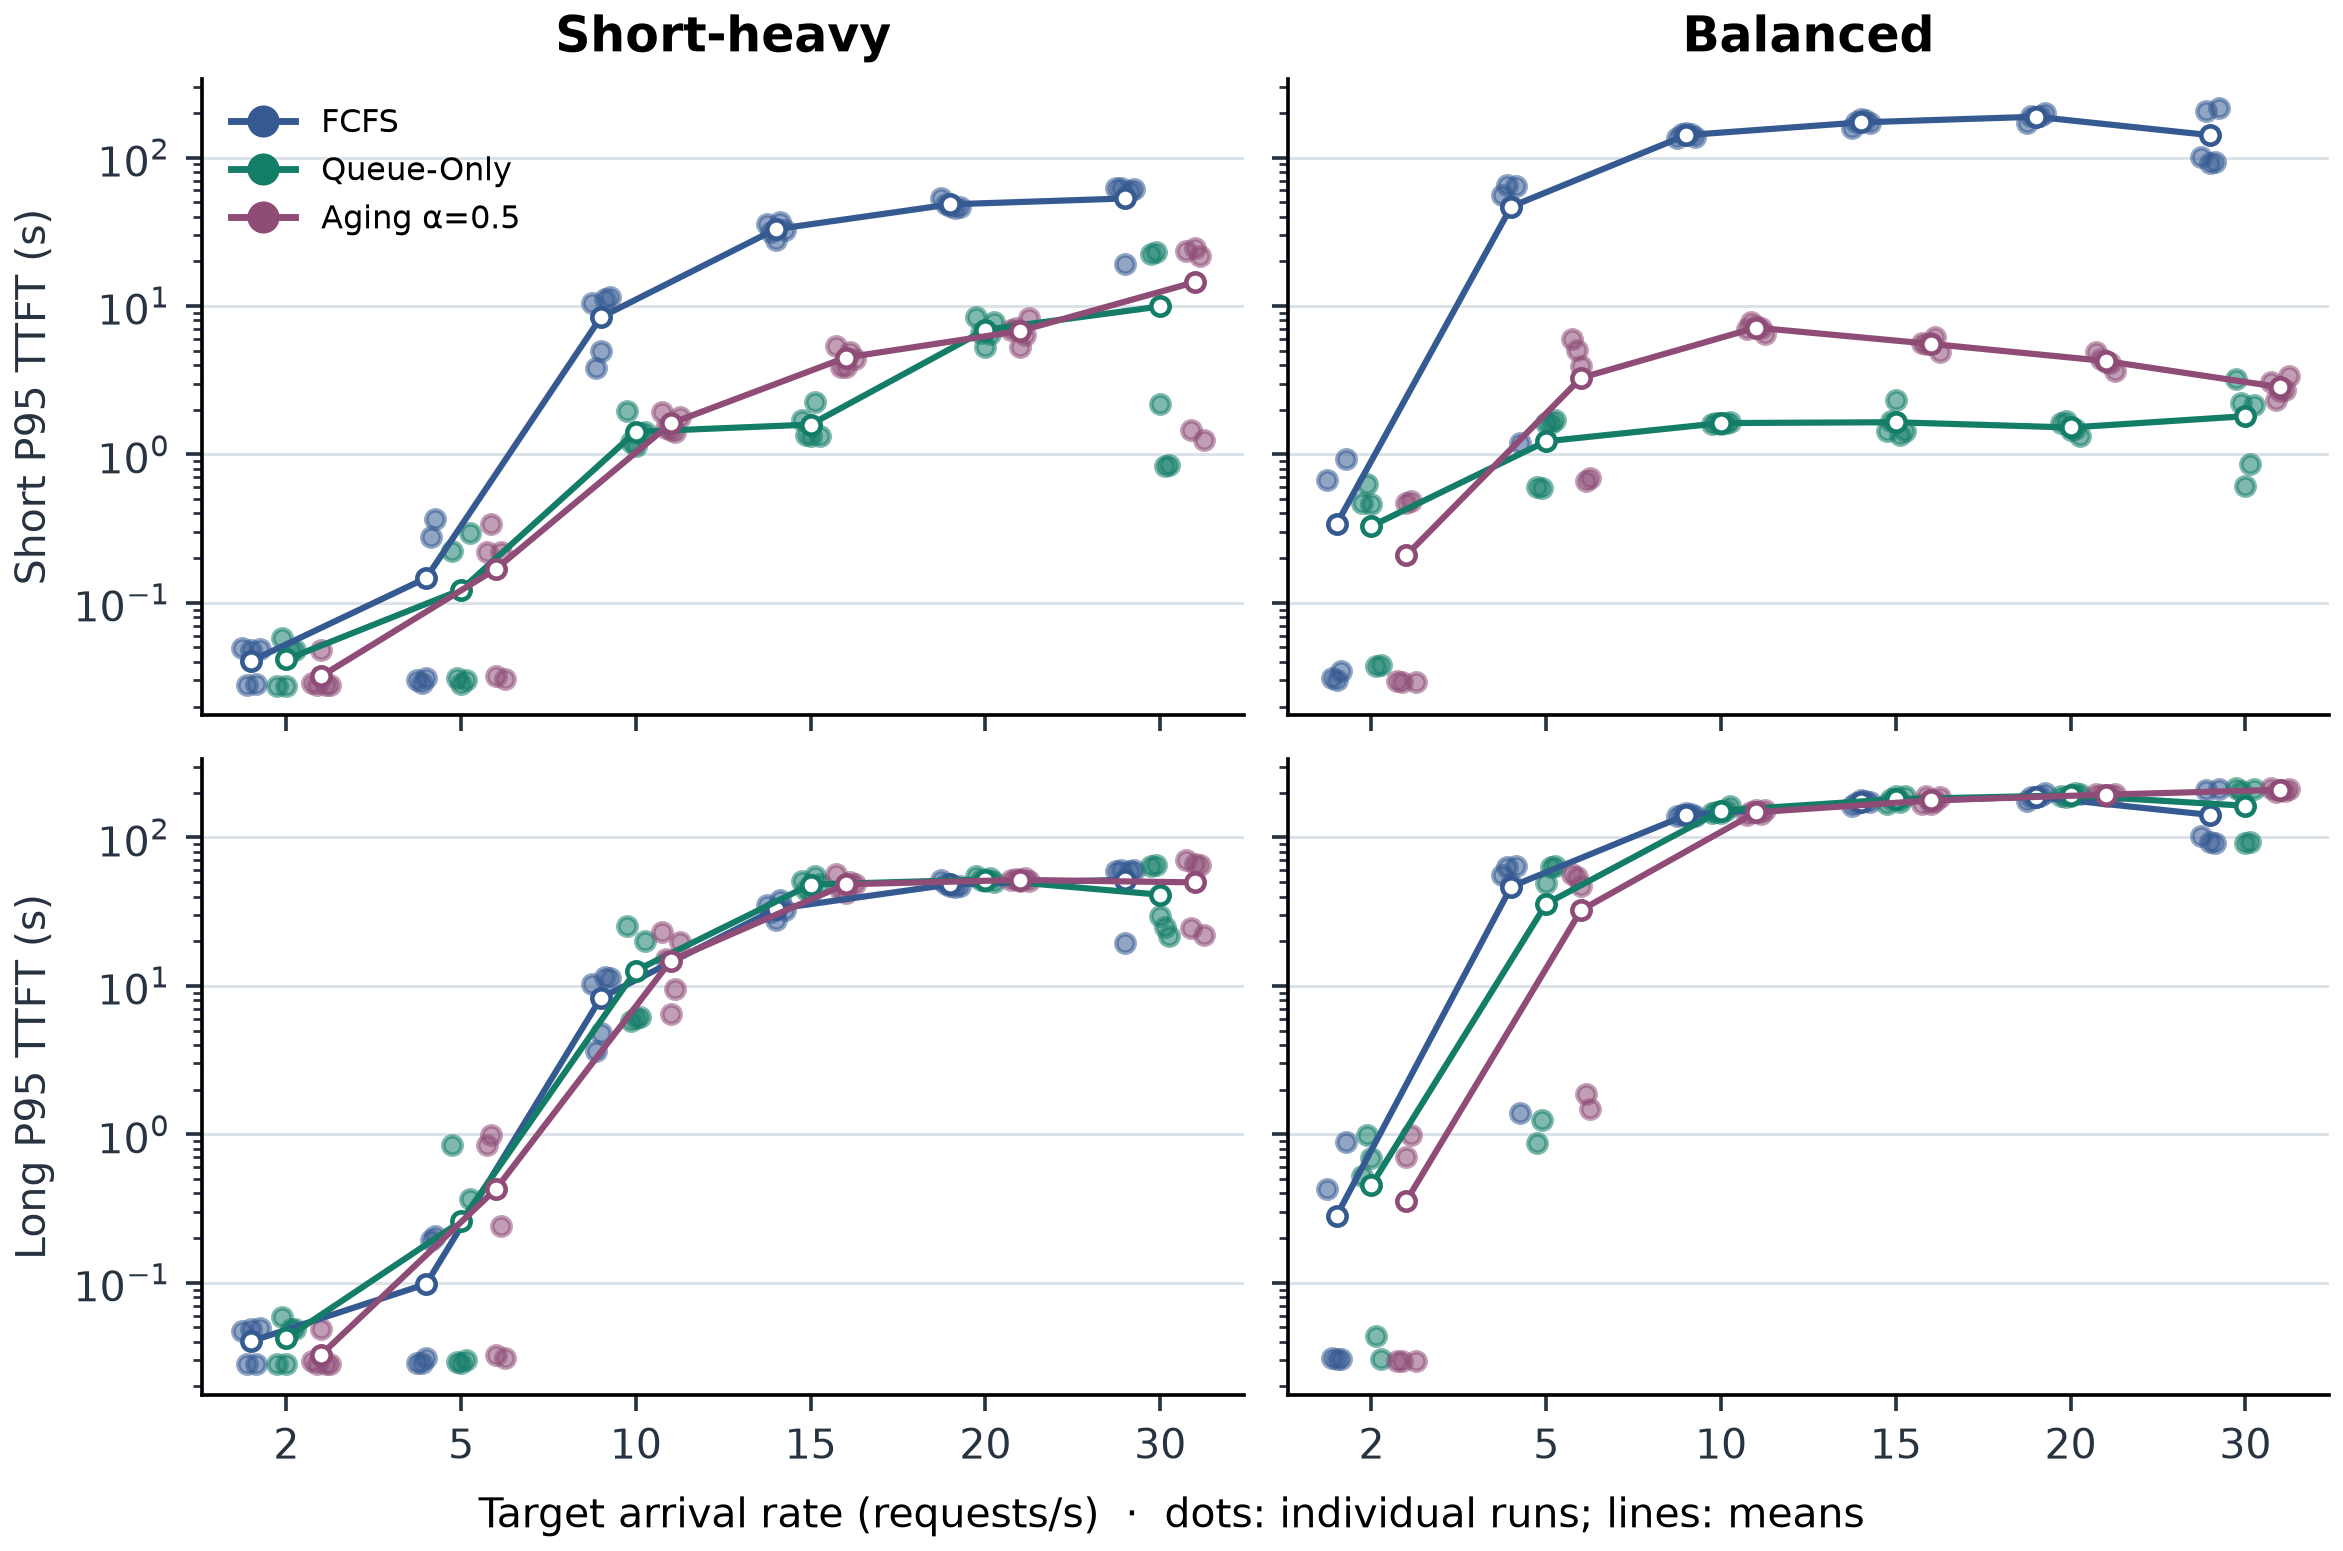
\includegraphics[width=0.89\textwidth]{modal_ttft_by_load.png}
\caption{Client P95 TTFT at cap 4. Faint dots are individual repetitions
and connected markers show means of five per-run P95 values. The vertical
axes are logarithmic and the horizontal axis lists target rates.}
\label{fig:ttft}
\end{figure*}

\subsection{Latency Across Load and Request Mix}

Figure~\ref{fig:ttft} shows that the effect depends on the backlog.
At 2 requests/s, the differences are small. At 5 requests/s,
FCFS mean server queue time is about 16 ms for the short-heavy mix and
25.90 s for the balanced mix. In the balanced case, Queue-Only
lowers mean short P95 TTFT from 46.79 to 1.23 s, and Aging yields
3.28 s. Aging's mean long P95 is 32.45 s versus 35.78 s for
Queue-Only. This average improvement in long latency is specific
to the condition and the pooled runs.

For balanced traffic at 10--20 requests/s, Queue-Only's mean
short P95 is 1.52--1.65 s, compared with 141.63--188.41 s for
FCFS. Long P95 rises by 4.13--10.15 s under Queue-Only.
At 30 requests/s, Queue-Only reduces short P95 in all five
balanced trace pairs. Its mean falls from 141.53 to 1.81 s.
Aging reaches 2.84 s. Long-request and throughput estimates at
30 requests/s vary with the execution environment, as discussed below.

\subsection{Admission Capacity and Workload Sensitivity}

At balanced 5 requests/s, replaying the same five traces with caps
of 16, 64 and 256 yields mean short and long P95 values below
60 ms for every policy (Figure~\ref{fig:caps}). At cap 16, the
four FCFS pairs with matching logged GPU environments move from
46.85--64.93 s short P95 at cap 4 to 49--54 ms. This supports a
strong dependence on the admission cap for this workload.

At 5 requests/s, the result also changes with request composition
(Table~\ref{tab:workload}). At 10\% short requests, Queue-Only
reduces short P95 from 143.47 to 1.45 s and raises long P95 from
142.84 to 175.64 s. For lognormal lengths, short and medium
P95 under Queue-Only are 0.50 and 0.96 s, and long P95 is
52.71 s versus 49.29 s for FCFS. Burst arrivals preserve a large
short-latency benefit. The burst and original Poisson cases
use different trace seeds, so their results describe separate workloads.

The policy-variant sweep at balanced 5 requests/s shows no monotonic
relationship between Aging strength and pooled long P95. Wait Promotion
has 14.07 s short P95 and 15.22 s long P95. The noisy length variant has
1.13 s short P95 and 73.22 s long P95. Under the two-size workload,
the $\pm30\%$ perturbation leaves the length ranges disjoint, so it
reorders requests within each class. Per-variant environment labels
and all repetitions are retained in the artifact
(Table~\ref{tab:variants}).

\subsection{Long-Request Stress Test}

Each trace sends 888 short requests and 12 early long probes at a
30 requests/s target. All probes eventually complete in this finite
experiment. Of 60 long probes per policy, the number receiving their
first token after the last short send is 0 for FCFS and 59 for each
length-aware policy. Mean server queue times for long probes,
averaged over five runs, are 4.07 s for FCFS, 53.17 s for Queue-Only
and 56.89 s for Aging. Smooth aging at $\alpha=0.5$ did not provide
effective long-request protection in this workload.

\subsection{Scheduler Cost and Throughput}

At balanced 30 requests/s, profiled FCFS, Queue-Only and Aging
take 99, 210 and 303 $\mu$s per scheduler call on average.
The queue-reordering path accounts for 49\% of Queue-Only and
63\% of Aging scheduler CPU time. For calls with at least 100
waiting requests, the shares rise to 54\% and 67\%. Skipping
unchanged queue rewrites yields 309 $\mu$s per call, compared with
303 $\mu$s for original Aging, on five trace pairs with the same
logged GPU environments. The mean throughput is 273.5 versus
273.2 generated tokens/s. We observed no speedup from this change.

The profiled policies averaged about 3.92 scheduled sequences per
nonempty step and 67\% prompt tokens among scheduled tokens.
These measurements describe batch composition. They do not
identify the fraction of GPU execution time spent in each phase.
Mean sampled GPU utilization ranges from roughly 15\% to 28\% across individual profiled runs.

At 30 requests/s, the unprofiled runs using driver 610.57.04 with
49,140 MiB visible GPU memory reach 433--499 generated tokens/s,
while those using driver 620.70.06 with 46,068 MiB reach
234--263 tokens/s (Figure~\ref{fig:throughput}). In balanced traffic,
after matching the trace and these GPU labels, Queue-Only differs
from FCFS by +3.60 tokens/s and $-0.82$ s long P95 on four pairs.
For Aging the corresponding changes are +5.16 tokens/s and
$-2.59$ s on two pairs. These small subsets support a descriptive
comparison and leave the source of the environment difference open.

\begin{figure*}[t]
\centering
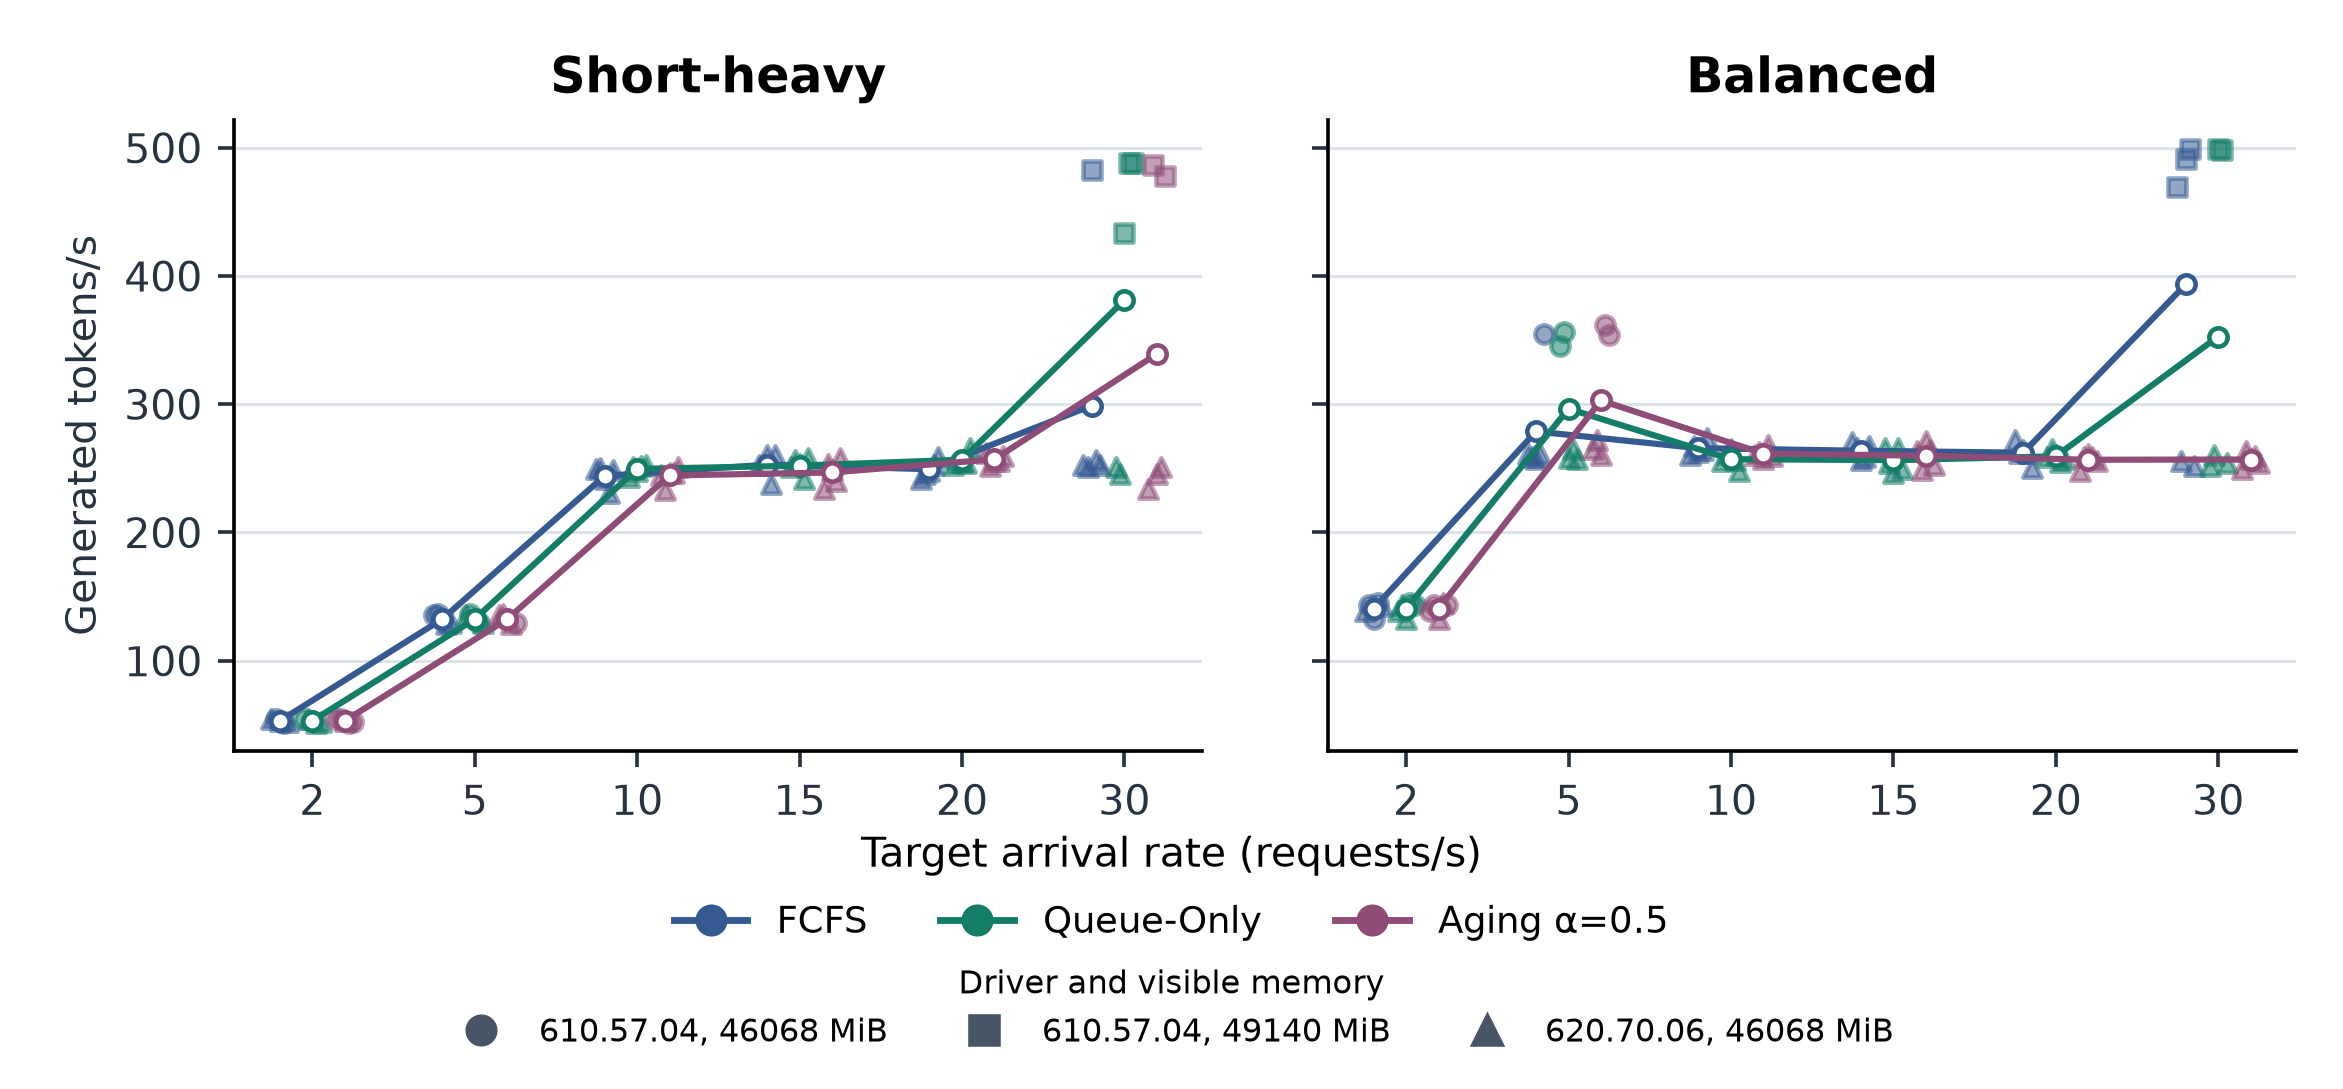
\includegraphics[width=0.86\textwidth]{modal_throughput_by_load.png}
\caption{Generated-token throughput by target rate at cap 4. Marker
shape on the individual runs records the NVIDIA driver and visible GPU
memory. Connected means pool environments.}
\label{fig:throughput}
\end{figure*}

\section{Limitations and Conclusion}

The experiments use one small model, synthetic workload traces and a
single-GPU server per run. The driver and visible-memory labels only
partially describe the execution environment. With five repetitions
per condition, we show the individual observations and avoid
claims of statistical significance. The stress test covers a finite
arrival window. Profiling snapshots are cumulative and may omit the
last partial block of 128 nonempty steps.

At a tight admission cap, length-aware queue ordering can give short
requests substantially better tail latency. The gain largely disappears
when the server can keep up with the offered work. Smooth aging changes
the trade-off, with nearly all long probes still delayed past the last short send
under sustained short arrivals. Deployments should evaluate latency
targets by request class and measure the cost of queue ordering under
their actual admission settings.

\begin{thebibliography}{9}

\bibitem{kwon2023efficient}
Woosuk Kwon, Zhuohan Li, Siyuan Zhuang,
Ying Sheng, Lianmin Zheng, Cody Hao Yu,
Joseph E. Gonzalez, Hao Zhang, and Ion Stoica.
2023.
Efficient Memory Management for Large Language
Model Serving with PagedAttention.
In \emph{Proceedings of the 29th Symposium
on Operating Systems Principles (SOSP '23)}.
ACM, 611--626.
\url{https://doi.org/10.1145/3600006.3613165}.

\bibitem{yu2022orca}
Gyeong-In Yu, Joo Seong Jeong, Geon-Woo Kim,
Soo-Young Kim, and Byung-Gon Chun.
2022.
Orca: A Distributed Serving System for
Transformer-Based Generative Models.
In \emph{Proceedings of the 16th USENIX
Symposium on Operating Systems Design
and Implementation (OSDI '22)}.
USENIX Association, 521--538.
\url{https://www.usenix.org/conference/osdi22/presentation/yu}.

\bibitem{agrawal2024sarathi}
Amey Agrawal, Nitin Kedia, Ashish Panwar,
Jayashree Mohan, Nipun Kwatra,
Bhargav S. Gulavani, Alexey Tumanov,
and Ramachandran Ramjee.
2024.
Taming Throughput-Latency Tradeoff
in LLM Inference with Sarathi-Serve.
In \emph{Proceedings of the 18th USENIX
Symposium on Operating Systems Design
and Implementation (OSDI '24)}.
USENIX Association.
\url{https://www.usenix.org/conference/osdi24/presentation/agrawal}.

\bibitem{sun2024llumnix}
Biao Sun, Ziming Huang, Hanyu Zhao, Wencong Xiao,
Xinyi Zhang, Yong Li, and Wei Lin. 2024.
Llumnix: Dynamic Scheduling for Large Language Model Serving.
In \emph{Proceedings of the 18th USENIX Symposium on Operating Systems
Design and Implementation (OSDI '24)}.
\url{https://www.usenix.org/conference/osdi24/presentation/sun-biao}.

\bibitem{bari2025optimal}
Agrim Bari, Parikshit Hegde, and Gustavo de Veciana. 2025.
Optimal Scheduling Algorithms for LLM Inference: Theory and Practice.
\emph{Proceedings of the ACM on Measurement and Analysis of Computing Systems}
9, 3, Article 59.
\url{https://arxiv.org/abs/2508.01002}.
\end{thebibliography}

\appendix

\section{Worked Example}
\label{app:example}

Consider request A with 256 prompt tokens, 128 maximum output tokens,
and 20 seconds in the queue. Requests B and C each have 32 prompt
tokens, 16 maximum output tokens and one second of waiting.
FCFS selects A first. Queue-Only scores A at 384 and B and C at 48,
so B and C have priority. With $\alpha=0.5$, Aging scores A at
$384/(1+0.5\cdot20)=34.91$ and B and C at $48/(1+0.5)=32$.
A's longer wait narrows the gap. For a newly arrived short request
scored at 48, A would take priority within the same waiting queue.
When two requests have the same score and arrival time, stable sorting
keeps their relative order.

\section{Detailed Results}

\begin{figure}[H]
\centering
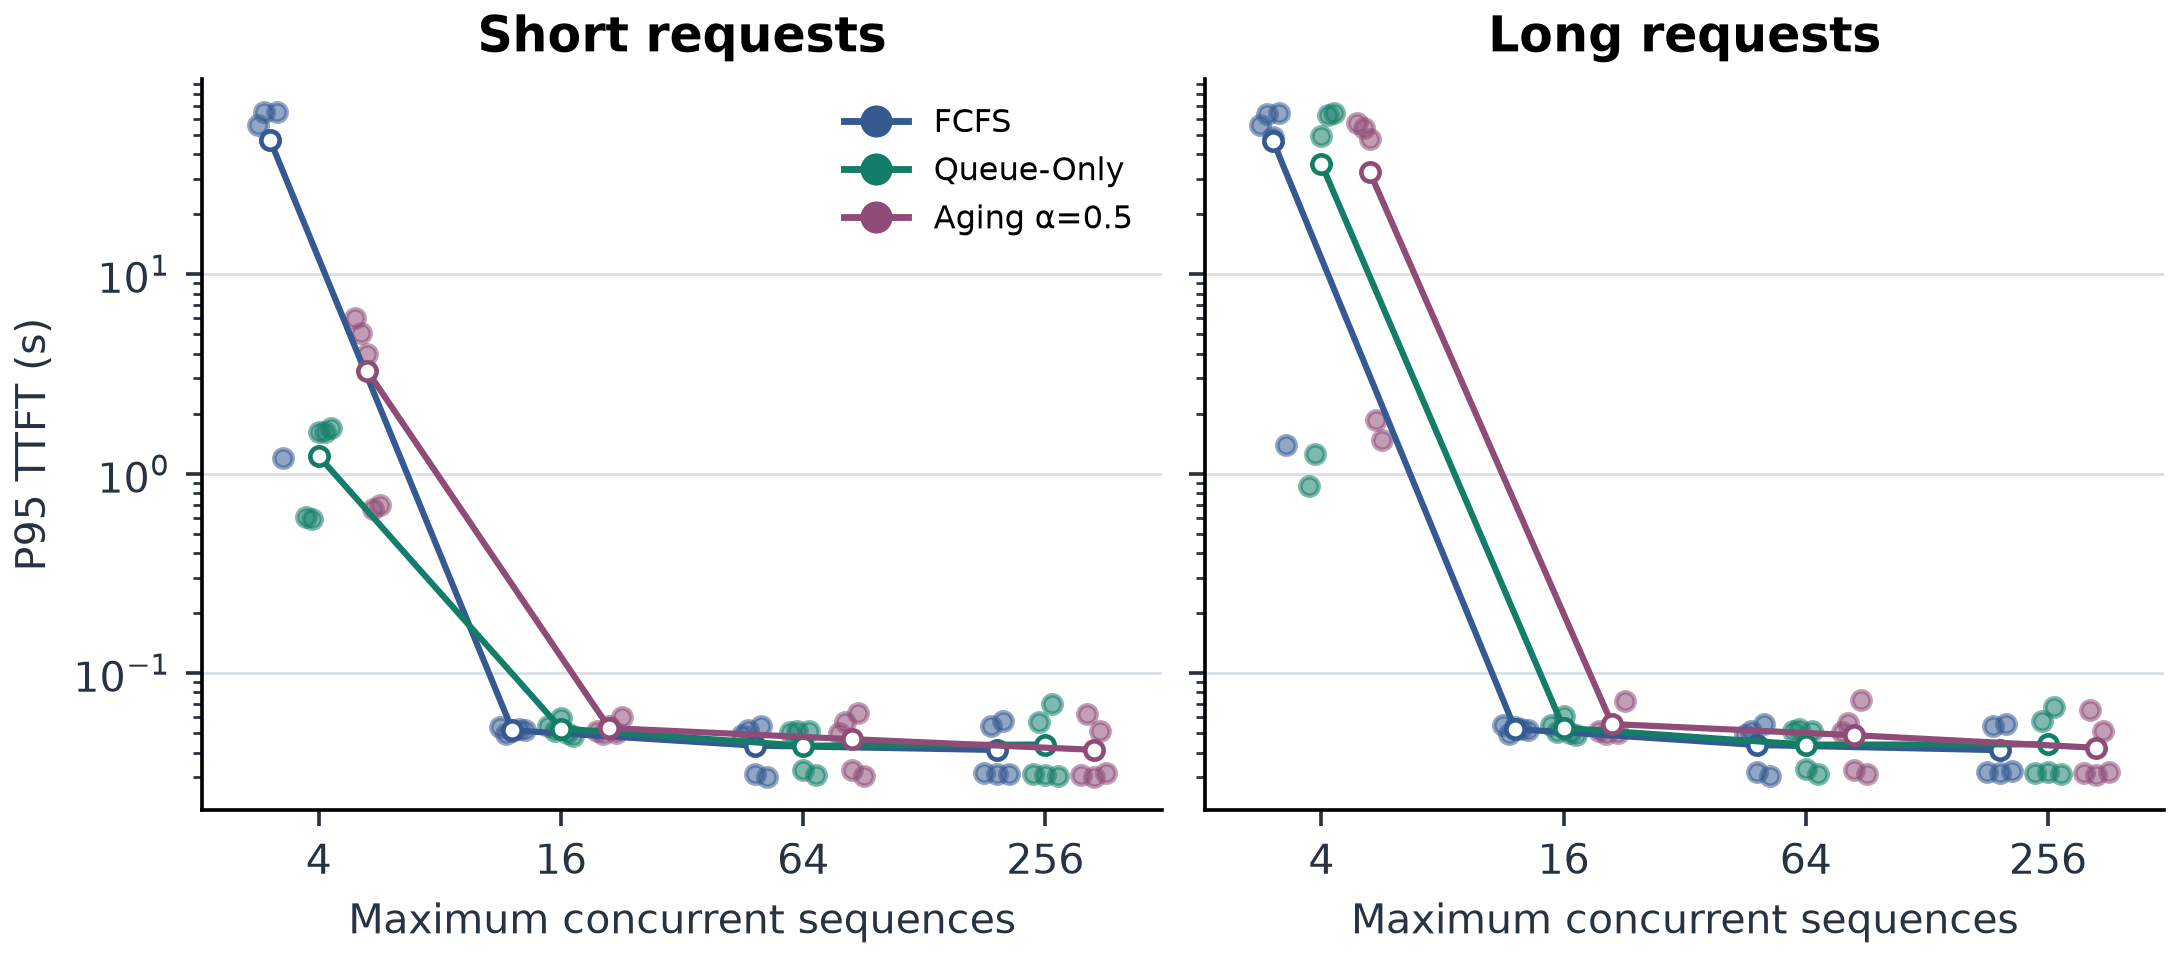
\includegraphics[width=\columnwidth]{modal_cap_sensitivity.png}
\caption{Balanced, 5 requests/s. A larger sequence cap nearly
eliminates waiting in this workload. Each point is one of five repeats.}
\label{fig:caps}
\end{figure}



\begin{table}[H]
\centering
\caption{Workload-sweep P95 TTFT. Each cell gives mean short / long
seconds over five runs at 5 requests/s and cap 4.}
\label{tab:workload}
\scriptsize
\setlength{\tabcolsep}{3pt}
\begin{tabular}{@{}lrrr@{}}
\toprule
Workload & FCFS & Queue-Only & Aging \\
\midrule
10\% short & 143.47 / 142.84 & 1.45 / 175.64 & 10.06 / 193.65 \\
30\% short & 109.86 / 110.13 & 1.38 / 86.68 & 7.67 / 121.35 \\
70\% short & 5.85 / 5.71 & 0.80 / 3.13 & 1.58 / 12.67 \\
Lognormal & 48.97 / 49.29 & 0.50 / 52.71 & 5.08 / 51.20 \\
Bursty balanced & 44.19 / 43.85 & 1.44 / 37.98 & 5.56 / 59.39 \\
\bottomrule
\end{tabular}
\end{table}

\begin{table}[H]
\centering
\caption{Policy variants, balanced at 5 requests/s with cap 4.
Values are mean per-run P95 TTFT in seconds ($n=5$ per row).}
\label{tab:variants}
\small
\begin{tabular}{@{}lrr@{}}
\toprule
Policy & Short & Long \\
\midrule
FCFS & 46.79 & 46.72 \\
Queue-Only & 1.23 & 35.78 \\
Aging $\alpha=0.5$ & 3.28 & 32.45 \\
vLLM native priority & 1.06 & 24.64 \\
Prompt-only & 0.70 & 1.55 \\
Noisy length & 1.13 & 73.22 \\
Aging $\alpha=1$ & 0.67 & 1.48 \\
Aging $\alpha=2$ & 2.06 & 14.97 \\
Aging $\alpha=5$ & 0.66 & 1.50 \\
Aging $\alpha=10$ & 3.16 & 22.24 \\
Wait Promotion & 14.07 & 15.22 \\
HRRN & 2.28 & 16.67 \\
\bottomrule
\end{tabular}
\end{table}

\section{Artifact and Reproduction}

The source repository is
\url{https://github.com/Car1eano/fall26-cs598ape-llm-length-aware-scheduling}.
\texttt{gpu\_experiments/} contains scheduler implementations and
the Modal launch instructions in \texttt{ENVIRONMENT.md}.
\texttt{benchmarks/} contains the request client and audit code.
\texttt{workload/} generates the deterministic workload traces.
Each result directory retains the planned blocks, audit journal,
request traces, GPU and package metadata, flags, and run artifacts.

The primary experiment requires an authenticated Modal environment
with L40S capacity. The local runner can launch the 90-run
main plan as follows. The drivers in \texttt{scripts/} run the intermediate arrival rates,
policy and cap sweeps, profiling, workload variations and the
starvation test. The full command sequence is documented in
\texttt{gpu\_experiments/ENVIRONMENT.md}.

\begin{lstlisting}
.venv/bin/modal run -m gpu_experiments.modal_smoke --formal
\end{lstlisting}

The aggregated CSVs are in \texttt{results/modal\_analysis/}. The
individual-runs table includes P50/P95/P99 TTFT and end-to-end
latency, generated-token throughput, queue summaries and TTFT
service-level attainment. Paired deltas include both GPU environment
labels. The plot script rebuilds Figures~\ref{fig:ttft},
\ref{fig:caps} and~\ref{fig:throughput} from that CSV.

\begin{lstlisting}
.venv/bin/python -m report_analysis.plot_modal_results \
  results/modal_analysis/individual_runs.csv \
  --out report/figures
.venv/bin/tectonic --untrusted --outdir output/pdf \
  report/final_report.tex
\end{lstlisting}

\end{document}
